\chapter{TINJAUAN PUSTAKA}
\label{chap:tinjauanpustaka}

% Ubah bagian-bagian berikut dengan isi dari tinjauan pustaka

\section{Hasil penelitian/perancangan terdahulu }
\label{sec:roketluarangkasa}

% Contoh input gambar
% \begin{figure}[ht]
%   \centering

%   % Ubah dengan nama file gambar dan ukuran yang akan digunakan
%   \includegraphics[scale=0.35]{gambar/roketluarangkasa.jpg}

%   % Ubah dengan keterangan gambar yang diinginkan
%   \caption{Peluncuran roket luar angkasa \emph{Discovery} \parencite{roketluarangkasa}.}
%   \label{fig:roketluarangkasa}
% \end{figure}

Beberapa penelitian yang terkait dengan penjadwalan dan algoritma genetika adalah 
\linebreak penelitian yang dilakukan oleh Ardiansyah dan Junianto (2022) 
dengan judul Penerapan \linebreak Algoritma Genetika untuk Penjadwalan Mata Pelajaran. 
Dari penelitian ini dihasilkan kesimpulan bahwa proses penjadwalan mata pelajaran dengan 
aplikasi penjadwalan yang menggunakan algoritma genetika jauh lebih efisien daripada 
dilakukan dengan cara semi manual dengan bantuan google sheet. Penggunaan aplikasi 
penjadwalan juga menghasilkan keluaran file yang sama dengan metode semi-manual yaitu berbentuk excel.

Selanjutnya pada penelitian yang dilakukan Alnowaini dan Aljomai (2021) dengan judul penelitian 
Genetic Algorithm for Solving University Course Timetabling Problem Using Dynamic Chromosomes 
yang dipublikasikan pada International Conference of Technology, Science and Administration 2021 
diperoleh hasil penggunaan algoritma genetika untuk proses penjadwalan perkuliahan terbukti efisien 
dengan mendapatkan nilai fitness function sebesar 24.0 dan dengan waktu pembuatan jadwal 5 menit. 
Hasil penjadwalan mendekati nilai optimal untuk ditetapkan pada perkuliahan di 3 departemen 
(Information Technology, Communication, Computer Networks, and Distribution Systems) Taiz University, Yaman. 
Waktu penjadwalan berkurang drastis dengan pengaplikasian algoritma genetika.

Mone dan Simarmata (2021) melakukan penelitian dengan judul 
Aplikasi Algoritma \linebreak Genetika Dalam Penjadwalan Mata Kuliah mendapatkan hasil 
penjadwalan berhasil dilakukan dengan running aplikasi diperoleh rata-rata waktu eksekusi 
30 jadwal adalah 25.86 menit, standar deviasi 11,88 menit dengan jumlah ruang kuliah sebanyak 3 
ruang kuliah, dan 1 ruang aula untuk mata kuliah umum, 51 pengampu mata kuliah, 18 dosen, 5 hari 
kerja dan 14 jam efektif per hari. Selain itu jadwal yang dihasilkan tidak terjadi bentrok dosen, 
tidak terjadi bentrok ruang dan waktu, tidak terjadi bentrok waktu dosen yang berhalangan, 
dan tidak terjadi bentrok dengan waktu sholat jumat. Dari hasil-hasil tersebut disimpulkan 
bahwa aplikasi penjadwalan yang dibuat efektif dan efisien.

\section{Teori/Konsep Dasar}
\label{sec:teori}
\subsection{Penjadwalan}
\label{subsec:penjadwalan}
Penjadwalan merupakan proses perencanaan untuk menentukan kapan dan dimana setiap \linebreak kegiatan sebagai bagian dari pekerjaan secara keseluruhan harus dilakukan pada sumber daya yang terbatas, serta pengalokasian sumber daya pada suatu waktu tertentu dengan memperhatikan kapasitas sumber daya yang ada. 
Penjadwalan dapat diartikan sebagai pengalokasian sejumlah sumber daya (resource) untuk melakukan sejumlah tugas atau operasi dalam jangka waktu tertentu dan merupakan proses pengambilan keputusan yang peranannya sangat penting. 
Penjadwalan juga dapat didefinisikan sebagai proses pengalokasian sumber daya untuk mengerjakan sekumpulan tugas dalam jangka waktu tertentu dengan 2 arti penting sebagai berikut: 
\begin{enumerate}
  \item Penjadwalan merupakan suatu fungsi pengambilan keputusan untuk membuat atau \linebreak menentukan jadwal. 
  \item Penjadwalan merupakan suatu teori yang berisi sekumpulan prinsip dasar, model, teknik, dan kesimpulan logis dalam proses pengambilan keputusan yang memberikan pengertian dalam fungsi penjadwalan (\cite{prasetya2017penjadwalan}).
\end{enumerate}

\subsection{Algoritma Genetika}
\label{subsec:Algoritma}
Algoritma genetika ditemukan oleh John Holland pada tahun 1975 di Universitas Michigan, Amerika Serikat yang dipublikasikan dalam bukunya yang berjudul “Adaption in Natural and Artificial Systems”. 
Menurut John Holland, setiap masalah yang berbentuk adaptasi baik alami, maupun buatan dapat diformulasikan dalam terminologi genetika. Algoritma genetika merupakan algoritma pencarian heuristik yang didasarkan atas mekanisme seleksi alami dan genetika alami (\cite{Mauluddin2018}). 

Algoritma Genetika merupakan teknik untuk mencari solusi optimal dari permasalahan yang memiliki banyak penyelesaian. 
Teknik ini akan melakukan pencarian dari beberapa solusi yang diperoleh hingga mendapatkan solusi terbaik sesuai dengan kriteria yang telah ditentukan atau yang disebut sebagai fungsi fitness. 
Algoritma ini masuk dalam kelompok algoritma evolusioner. Algoritma ini menggunakan pendekatan evolusi Darwin di bidang Biologi seperti pewarisan sifat, seleksi alam, mutasi gen dan kombinasi (crossover).  
Karena merupakan Teknik pencarian optimal dalam bidang ilmu komputer, maka algoritma ini juga termasuk dalam kelompok algoritma metaheuristik (\cite{binusAlgoritmaGenetika}).

Berikut ini adalah uraian singkat dari tahapan-tahapan dalam proses algoritma genetika:
\begin{enumerate}
  \item Skema Pengodean
  
  Dalam sebagian besar masalah komputasi, skema pengkodean yang merupakan metode untuk 
  mengubah data dalam bentuk tertentu memiliki peran yang amat penting. 
  Informasi yang diberikan dalam proses algoritma genetika harus dikodekan menjadi string bit tertentu. 
  Skema pengkodean ini dibedakan menurut domain masalah (\cite{Katoch2020}).
  
  Pada umumnya dikenal beberapa skema pendekodean kromosom, yaitu antara lain : 
  \begin{enumerate}
    \item Binary Encoding
      \begin{figure} [ht] \centering
        % Nama dari file gambar yang diinputkan
        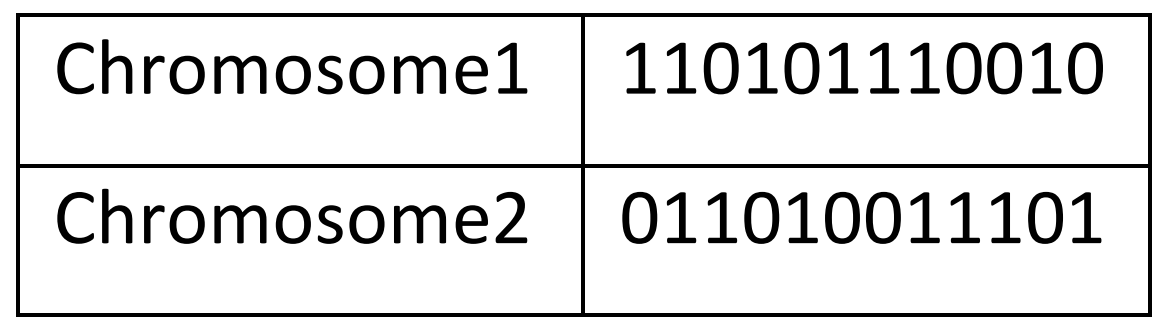
\includegraphics[scale=0.25]{gambar/binary.png}
        % Keterangan gambar yang diinputkan
        \caption{\emph{Binary encoding}}
        % Label referensi dari gambar yang diinputkan
        \label{fig:binary}
      \end{figure}

    Skema pengkodean ini merupakan skema pengkodean yang paling sering \linebreak digunakan. 
    Tiap gen atau kromosom direpresentasikan dengan angka 1 atau 0. Pada skema pengkodean biner, 
    tiap bit merepresentasikan karakteristik dari solusi. \linebreak Disisi lain, tiap biner juga merepresentasikan sebuah nilai.
    Metode ini membuat implementasi operasi crossover dan mutasi menjadi lebih cepat. 
    Metode crossover yang mungkin digunakan pada pengkodean biner adalah crossover 1 titik, crossover banyak titik, crossover uniform dan crossover aritmatika.
    Metode mutasi yang dapat digunakan pada pengkodean ini adalah mutasi flip.
    Dalam mutasi Flip, bit berubah dari 0 menjadi 1 dan 1 menjadi 0 berdasarkan kromosom mutasi yang dihasilkan.
    Namun skema pengkodean ini memerlukan proses yang lebih rumit karena harus mengonversi data menjadi kode biner dan akurasi dari algoritma ditentukan oleh proses konversinya (\cite{Katoch2020}).
    \item Octal Encoding
      \begin{figure} [ht] \centering
        % Nama dari file gambar yang diinputkan
        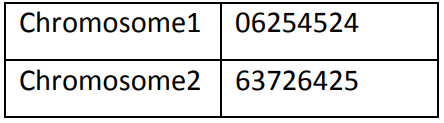
\includegraphics[scale=0.6]{gambar/octal.png}
        % Keterangan gambar yang diinputkan
        \caption{\emph{Octal encoding}}
        % Label referensi dari gambar yang diinputkan
        \label{fig:octal}
      \end{figure}

    Pada skema pengkodean oktal, gen atau kromosom direpresentasikan dalam bentuk angka oktal (0-7) (\cite{kumar2013encoding}).
    \item Hexadecimal Encoding
      \begin{figure} [ht] \centering
        % Nama dari file gambar yang diinputkan
        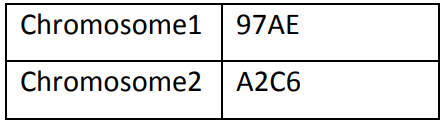
\includegraphics[scale=0.6]{gambar/hexa.png}
        % Keterangan gambar yang diinputkan
        \caption{\emph{Hexadecimal encoding}}
        % Label referensi dari gambar yang diinputkan
        \label{fig:hexa}
      \end{figure}

    Pada skema pengkodean heksadesimal, gen atau kromosom direpresentasikan dalam bentuk angka heksadesimal(0-9, A-F) (\cite{kumar2013encoding}).
    \item Permutation Encoding
      \begin{figure} [ht] \centering
          % Nama dari file gambar yang diinputkan
          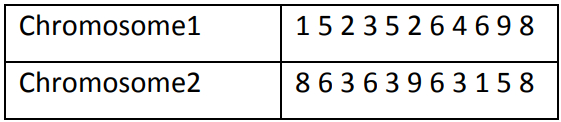
\includegraphics[scale=0.6]{gambar/permutation.png}
          % Keterangan gambar yang diinputkan
          \caption{\emph{Permutation encoding}}
          % Label referensi dari gambar yang diinputkan
          \label{fig:permutation}
        \end{figure}

        Pengkodean Permutasi digunakan dalam masalah pengurutan. 
        Dalam hal ini, setiap kromosom merepresentasikan posisi dalam sebuah urutan, misalnya dalam \emph{travelling salesman problem}, rangkaian angka merepresentasikan urutan kota yang dikunjungi oleh salesman.
        Terkadang, proses koreksi diperlukan setelah proses algoritma genetika dilakukan.(\cite{kumar2013encoding}). 
    \item Value Encoding

    Dalam skema pengkodean ini, gen atau kromosom direpresentasikan menggunakan string dari beberapa nilai. 
    Nilai-nilai ini bisa berupa bilangan real, bilangan bulat, atau karakter huruf. 
    Skema pengkodean ini dapat membantu dalam memecahkan masalah di mana nilai yang lebih rumit digunakan. 
    Karena pengkodean biner mungkin gagal dalam masalah seperti itu. 
    Metode encoding ini sering digunakan dalam \emph{neural network} untuk menemukan bobot optimal(\cite{Katoch2020}).
    \begin{figure} [!h] \centering
      % Nama dari file gambar yang diinputkan
      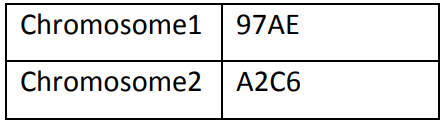
\includegraphics[scale=0.6]{gambar/hexa.png}
      % Keterangan gambar yang diinputkan
      \caption{\emph{Hexadecimal encoding}}
      % Label referensi dari gambar yang diinputkan
      \label{fig:hexa}
    \end{figure}
  \end{enumerate}
  
  \item Inisialiasi Populasi Awal
  
  Penentuan populasi awal merupakan proses pembuatan beberapa kromosom secara acak. Kromosom adalah solusi alternatif yang mungkin. Dapat dikatakan bahwa kromosom sama dengan individu. Besar kecilnya populasi tergantung pada masalah yang akan dipecahkan. Setelah menentukan ukuran populasi, populasi awal dibentuk dengan memulai kemungkinan solusi untuk kromosom yang berbeda. Panjang kromosom ditentukan berdasarkan masalah yang dipelajari(\cite{Ardiansyah2022}).
  \item Fungsi Fitness
  
  Individu dievaluasi berdasarkan fungsi tertentu sebagai ukuran kinerjanya. 
  Individu dengan nilai fitness tinggi pada kromosomnya yang akan dipertahankan, 
  sedangkan individu yang pada kromosomnya bernilai fitness rendah akan diganti. 
  Fungsi fitness tergantung pada permasalahan tertentu dari representasi yang digunakan. 
  Secara umum perhitungan nilai fitness dari setiap kromosom dapat dirumuskan sebagai berikut.
  \begin{equation}
    \label{eq:fitness}
    \mathbf{Fitness} = \frac{1}{1 + (F1B1 + F2B2 + \cdot \cdot \cdot +  FnBn)}\; 
  \end{equation}

  Keterangan :\\
  Bn = Bobot Pelanggaran\\
  Fn = Banyaknya Pelanggaran\\
  n  = 1…n (\cite{muhammad2020penjadwalan})
  \item Seleksi
  
  Seleksi merupakan proses yang penting dalam algoritma genetika. 
  Prosesn seleksi akan menentukan apakah sebuah individu akan berpartisipasi dalam proses reproduksi atau tidak.
  Proses seleksi ini juga biasa dikenal sebagai operator reproduksi. 
  Teknik seleksi yang umum digunakan pada algoritma genetika antara lain \emph{roulette wheel, rank, tournament, boltzmann,} dan \emph{stochastic universal sampling}.(\cite{Katoch2020}).
  
  \begin{enumerate}
    \item \emph{Roulette wheel}
    

    Metode \emph{roulette wheel} memetakan semua individu sesuai dengan nilai probabilitasnya. Probabilitas ini ditentukan berdasarkan nilai fitnessnya. Individu tersebut dipetakan ke dalam roda, kemudian diputar secara acak untuk menentukan individu mana yang akan berpartisipasidalam pembentukan generasi berikutnya(\cite{Katoch2020}.)
    
    \begin{figure} [!h] \centering
      % Nama dari file gambar yang diinputkan
      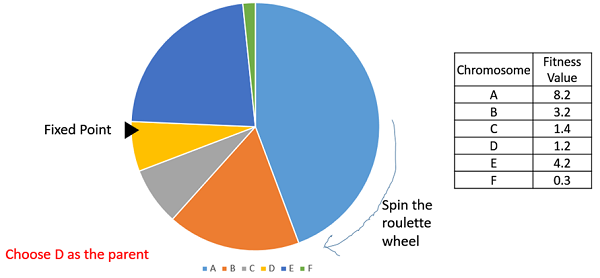
\includegraphics[scale=0.6]{gambar/roulette_wheel_selection.jpg}
      % Keterangan gambar yang diinputkan
      \caption{\emph{Roulette wheel selection}}
      % Label referensi dari gambar yang diinputkan
      \label{fig:roulette}
    \end{figure}

    \item \emph{Rank}
    
    Metode \emph{rank} merupakan modifikasi dari metode \emph{roulette wheel}. Metode ini menggunakan ranking dari masing-masing individu berdasarkan nilai fitnesnya. Metode ini mengurangi kemungkinan konvergensi solusi sebelum waktunya(\cite{Katoch2020}).
    
    \begin{figure} [ht] \centering
      % Nama dari file gambar yang diinputkan
      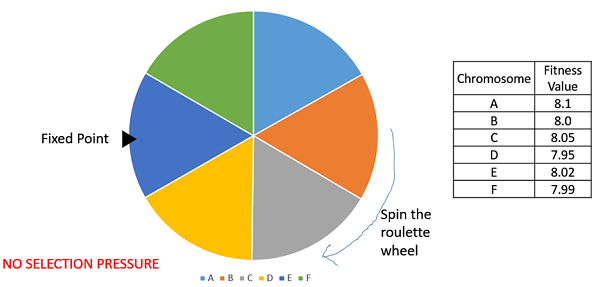
\includegraphics[scale=0.55]{gambar/rank_selection.jpg}
      % Keterangan gambar yang diinputkan
      \caption{\emph{Rank selection}}
      % Label referensi dari gambar yang diinputkan
      \label{fig:rank}
    \end{figure}

    \item \emph{Tournament} 
    
    \begin{figure} [ht] \centering
      % Nama dari file gambar yang diinputkan
      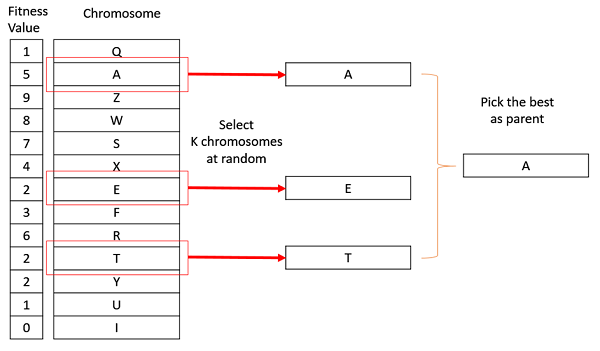
\includegraphics[scale=0.6]{gambar/tournament_selection.jpg}
      % Keterangan gambar yang diinputkan
      \caption{\emph{Tournament selection}}
      % Label referensi dari gambar yang diinputkan
      \label{fig:tournament}
    \end{figure}

    Teknik pemilihan \emph{tournament} pertama kali diusulkan oleh Brindle pada tahun 1983. Individu dipilih berdasarkan nilai fitness mereka pada \emph{stochastic roulette wheel} secara berpasangan. Setelah seleksi,
    individu dengan nilai fitness yang lebih tinggi akan ditambahkan ke \emph{pool} generasi berikutnya(\cite{Katoch2020}).
    \item \emph{Boltzmann} 
    
    Metode seleksi \emph{Boltzmann} merupakan metode seleksi yang berbasis entropy dan metode sampling, yang digunakan pada \emph{Monte
    Carlo Simulation}. Metode ini membantu dalam memecahkan masalah konvergensi prematur(\cite{Katoch2020}).
    \item \emph{Stochastic Universal Sampling}
    
    \begin{figure} [ht] \centering
      % Nama dari file gambar yang diinputkan
      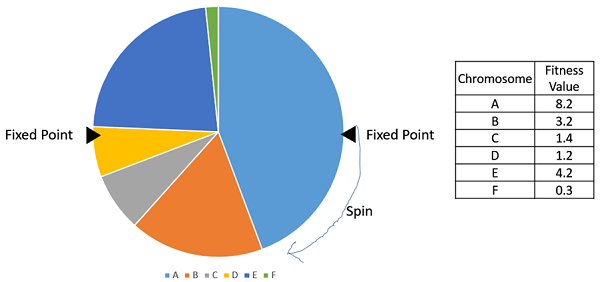
\includegraphics[scale=0.6]{gambar/sus.jpg}
      % Keterangan gambar yang diinputkan
      \caption{\emph{Stochastic Universal Sampling}}
      % Label referensi dari gambar yang diinputkan
      \label{fig:SUS}
    \end{figure}
    \emph{Stochastic Universal Sampling} merupakan pengembangan dari metode \emph{roulette \linebreak wheel}. Pada metode ini, posisi tiap individu ditentukan secara acak dengan jarak yang sama antar satu dengan yang lain. Dengan metode ini semua individu memiliki kesempatan yang sama untuk terpilih(\cite{Katoch2020}).
  \end{enumerate}
  \item Crossover
  
  Crossover (Persilangan) adalah sebuah proses
  yang membentuk kromosom baru dari dua
  kromosom induk dengan menggabungkan
  bagian informasi dari masing-masing kromosom
  Crossover menghasilkan kromosom baru
  yang disebut kromosom anak (\emph{offspring}).
  Crossover bertujuan untuk menambah
  keanekaragaman string dalam satu populasi
  dengan penyilangan antar string yang diperoleh
  dari reproduksi sebelumnya. Hasil crossover 2
  kromosom induk akan menghasilkan 2 \emph{offspring}(\cite{JMASIF2649}).
  Ada beberapa metode yang bisa digunakan untuk melakukan crossover, antara lain:
  \begin{enumerate}[nolistsep]
    \item Single Point Crossover
    
    Metode ini merupakan metode crossover yang paling umum digunakan. 
    Pada \linebreak metode ini, satu titik persilangan dipilih secara acak di sepanjang kromosom yang disilangkan. 
    Kemudian bagian kepala dan ekor dari masing-masing induk ditukar antara satu sama lain. 
    Jika titik persilangan yang dipilih sesuai, maka offspring yang dihasilkan akan menjadi lebih baik. 
    Sebaliknya jika titik yang dipilih salah, maka hal ini akan menghambat proses algoritma genetika menuju tujuannya (\cite{Kora}). 
    \item N-Point Crossover
    
    Crossover N-point pertama kali diimplementasikan oleh De Jong pada tahun 1975. 
    Crossover ini memiliki banyak titik crossover namun aturan yang digunakan sama dengan yang digunakan pada crossover satu titik. 
    Pada crossover 2 titik, titik \linebreak persilangan adalah 2. 
    Menambahkan lebih banyak titik crossover akan berdampak pada terganggunya blok-blok pembangun yang terkadang mengurangi kinerja\linebreak algoritma genetika. 
    Namun, hal ini memungkinkan bagian kepala dan ekor \linebreak kromosom untuk diterima secara bersamaan pada keturunannya (\cite{Kora}). 
    \item Uniform Crossover
    
    Pada uniform crossover,tidak dilakukan pemecahan kromosom untuk rekombinasi. 
    Setiap gen pada keturunan dibuat dengan cara menyalinnya dari induk yang dipilih sesuai dengan bit yang sesuai. 
    Crossover ini biasanya digunakan pada kromosom dengan binary encoding. 
    Crossover mask memiliki panjang yang sama dengan panjang kromosom induk. 
    Jika bit pada crossover mask adalah 1, maka gen yang dihasilkan disalin dari induk pertama dan jika bit pada crossover mask adalah 0, maka gen yang dihasilkan disalin dari induk kedua. 
    Crossover mask baru dibuat secara acak untuk setiap pasangan kromosom induk. 
    Jumlah titik crossover pada awalnya tidak ditetapkan. 
    Jadi, keturunannya memiliki campuran gen dari kedua orang tua (\cite{Kora}).
    \item Three Parent Crossover
    
    Dalam persilangan ini, tiga induk dipilih secara acak. 
    Setiap gen dari induk pertama dibandingkan dengan gen yang setara dari induk kedua. 
    Jika kedua gen serupa, gen tersebut digunakan untuk keturunannya, atau jika tidak, gen yang setara dari induk ke-3 diambil untuk keturunannya. 
    Metode ini seringkali digunakan dalam kasus kromosom yang menggunakan pengkodean biner (\cite{Kora}).
    \item Arithmetic Crossover
    
    Crossover aritmatika digunakan dalam kasus kromosom dengan real-value encoding. 
    Operator crossover aritmatika menggabungkan dua kromosom induk secara linear, dua kromosom tertentu secara acak untuk crossover dan membuat dua keturunan yang merupakan campuran linear dari orang tua mereka. (\cite{Kora})
  
    \item Partially Mapped Crossover
    
    Partially Matched atau Mapped Crossover (PMX) adalah metode crossover yang paling sering digunakan. 
    Diusulkan oleh Goldberg dan Lingle untuk Travelling Salesman Problem. 
    Dalam Partially Matched Crossover, dua kromosom \linebreak dihubungkan dan dua titik persilangan dipilih secara acak. 
    Fraksi kromosom antara dua titik crossover memberikan pilihan yang sesuai yang mengalami proses crossover melalui operasi pertukaran posisi per posisi (\cite{Kora}).
  
    \item Crossover ORDER (OX)
    
    Metode ini diusulkan oleh Davis dan juga digunakan untuk kromosom dengan \linebreak pengkodean permutasi. 
    Prosesnya dimulai dengan cara yang mirip dengan PMX dengan memilih dua titik persilangan. 
    Namun, alih-alih menggunakan pertukaran titik demi titik seperti pada PMX, order crossover menggunakan gerakan geser untuk mengisi lubang yang ditinggalkan dengan mengirimkan posisi yang dipetakan. 
    Metode ini menyalin bagian dari elemen permutasi antara titik-titik crossover dari string yang dipotong langsung ke keturunannya, menyisipkannya di posisi absolut yang sama (\cite{Kora}).
  
    \item Cycle Crossover (CX)
    
    Persilangan ini digunakan untuk kromosom dengan pengkodean permutasi. 
    Selama rekombinasi pada cyclic crossover terdapat batasan bahwa setiap gen berasal dari satu induk atau induk lainnya. 
    Model dasar pada cycle crossover adalah bahwa setiap alel berasal dari satu induk dengan posisi yang sama. 
    Untuk membuat siklus alel dari induk1, kita harus mulai dengan alel pertama dari induk1. 
    Kemudian lihat alel pada posisi yang sama di induk2 dan pergi ke posisi dengan alel yang sama di Induk1. 
    Masukkan alel ini ke dalam siklus dan lakukan lagi langkah di atas hingga mencapai pada alel pertama dari induk1. 
    Letakkan alel-alel dari siklus pada anak pertama pada posisi yang mereka miliki pada induk pertama dan alel-alel yang tersisa dari anak pertama berasal dari induk kedua beserta posisinya. 
    Proses ini diulangi untuk offspring ke 2 namun diawali dari induk 2 (\cite{Kora}).

  \end{enumerate}	
  
  \item Mutasi
  
  Mutasi adalah suatu modifikasi informasi gen-gen pada suatu kromosom. Proses mutasi dilakukan dengan pengkodean nilai yaitu memilih sembarang posisi gen pada kromosom, nilai yang ada tersebut kemudian diubah dengan suatu nilai tertentu yang diambil secara acak, memberikan nilai inversi atau menggeser nilai gen pada gen yang terpilih untuk dimutasikan(\cite{JMASIF2649}).
  \item Kriteria Penghentian
  
  Kriteria berhenti adalah kriteria yang digunakan untuk menghentikan proses algoritma genetika, yang merupakan tujuan yang harus dicapai oleh proses tersebut dalam hal ini adalah untuk penjdwalan yang optimal. Ada beberapa kriteria terminasi yang dapat digunakan antara lain memberikan batasan jumlah iterasi, memberi batasan waktu proses, atau menghitung ada tidakna pergantian individu dalam populasi(\cite{Ardiansyah2022})
\end{enumerate}

% Gravitasi merupakan \lipsum[1]

% \subsection{Hukum Newton}
% \label{subsec:hukumnewton}

% Newton \parencite{newton1687} pernah merumuskan bahwa \lipsum[1]
% Kemudian menjadi persamaan seperti pada persamaan \ref{eq:hukumpertamanewton}.

% % Contoh pembuatan persamaan
% \begin{equation}
%   \label{eq:hukumpertamanewton}
%   \sum \mathbf{F} = 0\; \Leftrightarrow\; \frac{\mathrm{d} \mathbf{v} }{\mathrm{d}t} = 0.
% \end{equation}

% \subsection{Anti Gravitasi}
% \label{subsec:antigravitasi}

% Anti gravitasi merupakan \lipsum[1]
